\documentclass[10pt]{article}
\usepackage[polish]{babel}
\usepackage[utf8]{inputenc}
\usepackage[T1]{fontenc}
\usepackage{amsmath}
\usepackage{amsfonts}
\usepackage{amssymb}
\usepackage[version=4]{mhchem}
\usepackage{stmaryrd}
\usepackage{bbold}
\usepackage{graphicx}
\usepackage[export]{adjustbox}
\graphicspath{ {./images/} }

\title{LIGA MATEMATYCZNA \\
 GRUDZIEŃ 2011 \\
 SZKOŁA PONADGIMNAZJALNA }

\author{}
\date{}


\begin{document}
\maketitle
\section*{ZADANIE 1.}
Łąka w kształcie kwadratu ma powierzchnię 1 hektara. Swoje norki wykopało tam 2011 zajęcy (każdy ma jedną norkę). Po pewnym czasie pojawił się jeszcze jeden zając - samotnik, który nie chce mieć sąsiada bliżej niż 1 metr od swojej norki. Udowodnij, że może tam zamieszkać.

\section*{ZADANIE 2.}
Znajdź wszystkie funkcje \(f: \mathbb{R} \backslash\{0\} \rightarrow \mathbb{R}\) spełniające warunek

\[
f(x)+3 f\left(\frac{1}{x}\right)=\frac{2}{x}
\]

dla każdej liczby rzeczywistej \(x\) różnej od zera.

\section*{ZADANIE 3.}
Kwadrat podzielono na mniejszy kwadrat i trzy prostokąty, jak na rysunku. Czy trzy spośród tych czterech części mogą mieć taki sam obwód?\\
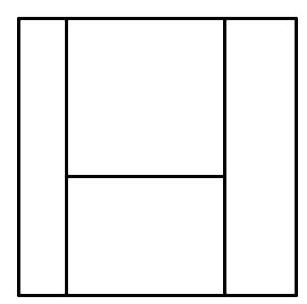
\includegraphics[max width=\textwidth, center]{2024_11_21_d5e73d8f56644ddda3d4g-1}

\section*{ZADANIE 4.}
Wykaż, że dla liczby całkowitej \(k\) liczba \(k^{6}-2 k^{4}+k^{2}\) jest podzielna przez 36.

\section*{ZADANIE 5.}
Wykaż, że wśród pięciu dowolnie wybranych liczb naturalnych zawsze znajdą się trzy takie, których suma jest podzielna przez 3.


\end{document}